\documentclass[10pt, a4paper]{article}
\usepackage[english,russian]{babel}
\usepackage{CJKutf8}
\usepackage[utf8]{inputenc}
\usepackage{multicol} %колонки
\usepackage{setspace} %межстрочный интервал
\usepackage{ragged2e}% выравнивания текста по ширине в документе.
\usepackage{fancyhdr} %настройки верхнего и нижнего колонтитулов в документе.
\usepackage{titlesec} %стилей заголовков разделов в документе.
\usepackage{enumitem} %настройки списков в документе.
\usepackage{graphicx}%Вставка картинок правильная
\usepackage{float}%"Плавающие" картинки
\usepackage{wrapfig}%Обтекание фигур (таблиц, картинок и прочего)
\usepackage[normalem]{ulem}
\usepackage{array}
\useunder{\uline}{\ul}{}

\usepackage[left=1.9cm,right=1.9cm, top=2.2cm,bottom=2.5cm]{geometry} % поля

\justifying % выравнивает текст по ширине.
\fancyhf{} %очищает все верхние и нижние колонтитулы.
\renewcommand{\headrulewidth}{0pt} % remove the header rule
\cfoot{\vskip -1.5cm \thepage} %устанавливает номер страницы в нижнем колонтитуле.

\linespread{0.8} %устанавливает межстрочный интервал в 0.84.

\setlength{\columnsep}{0.5cm}
\setcounter{page}{114}
\renewcommand{\thesection}{\Roman{section}} %устанавливает стиль нумерации разделов в виде заглавных римских цифр.

\titleformat{\section}{\footnotesize\centering\sc}{\thesection.}{0cm}{}[] %настраивает стиль заголовков разделов.

%%%%%%%%%%%%%%%%%%%%%%%%%%%%%%%%%%%%%
\renewcommand{\thesection}{\Roman{section}}
\setcounter{section}{5}
\usepackage[english, russian]{babel}

\begin{document}

\begin{multicols}{2}
\begin{center}


\section{  Classification of decision support systems}
\end{center}

\begin{flushleft}
DSS can be classified into 9 different classes in
accordance with the used information data, models and
knowledge. In table 1 structure formulae for each class of
DSS are represented [20].
\par
\begin{center}
\caption{ Таблица 1}
\end{center}
\begin{center}
\vspace{-\baselineskip}
  \vspace{0.1cm}
\caption{DSS classification}
\end{center}
\end{flushleft}
% Please add the following required packages to your document preamble:
% \usepackage[normalem]{ulem}
 %\useunder{\uline}{\ul}{} 

\begin{tabular}{|m{2.2cm}|m{2.2cm}|m{2.1cm}|} \hline
\scriptsize DSS structure formul                                                                                                                 & \scriptsize Information for decision making                                                                   & \scriptsize Used data, models and knowledge                                                                               \\ \hline
\begin{tabular}[c]{@{}l@{}} \footnotesize =objects+information \\ \scriptsize + information collection\\ \scriptsize tools\end{tabular}                                      &\scriptsize all which exists                                                                                  & \begin{tabular}[c]{@{}l@{}}\scriptsize all factual data \\ \scriptsize about \\ \scriptsize subject area\end{tabular}                                 \\ \hline
\scriptsize =alternatives+data + links                                                                                                         & \begin{tabular}[c]{@{}l@{}}\scriptsize all which can be\\ \scriptsize useful\end{tabular}                                 & \scriptsize actual data                                                                                                   \\ \hline
\scriptsize =alternatives + criteria + criteria’s values                                                                                         & \scriptsize all which is necessary (from that which exist)                                                    &\scriptsize  relevant (selected) data                                                                                      \\ \hline
\scriptsize =data + models                                                                                                                       &\scriptsize  all which can be formalized (modelled)                                                            &\scriptsize  formalized data (actual models)                                                                               \\ \hline
\scriptsize =models + rules criteria’s estimations                                                                                               &\scriptsize  all which must be modelled                                                                        & \scriptsize relevant models                                                                                               \\ \hline
\scriptsize =rules of alternatives’ estimation + alternatives’ rating                                                                            &\scriptsize  any variants                                                                                      & \begin{tabular}[c]{@{}l@{}}\scriptsize results of decision\\ \scriptsize  variant modelling \\ \scriptsize (actual knowledge)\end{tabular}            \\ \hline
\scriptsize =rules of alternatives’ choice + set of acceptable alternatives                                                                      & \scriptsize all the best (from that which exist)                                                              & \scriptsize relevant (generalized) knowledge                                                                              \\ \hline
\begin{tabular}[c]{@{}l@{}}\scriptsize =problem situations \\ \scriptsize + set of their\\\scriptsize  decisions examples \\ \scriptsize in the form of\\\scriptsize  subject collections\end{tabular} & \begin{tabular}[c]{@{}l@{}}\scriptsize all useful (about\\ \scriptsize  what formalized\\ \scriptsize  information exists)\end{tabular} & \begin{tabular}[c]{@{}l@{}}\scriptsize formalized\\ \scriptsize knowledge about\\ \scriptsize existing experience\\ \scriptsize  (precedent base)\end{tabular} \\ \hline
\scriptsize =inference system + best alternative                                                                                                 & \begin{tabular}[c]{@{}l@{}}\scriptsize best (possible)\\ \scriptsize variant\end{tabular}                                 & \begin{tabular}[c]{@{}l@{}}\scriptsize decision on the\\ \scriptsize base of digital\\ \scriptsize  intellectualizing\end{tabular} \\ \hline
\end{tabular}



\begin{flushleft}

\par
\small This classification allows creating a more efficient
enterprise business model. This is achieved mainly due
to the rational management of automation systems for
physical operations of production and related business
processes, integrated into united information space in
accordance with the key subsystems of the Industry
4.0 concept (Product Lifecycle Management, Big Data,
SMART Factory, cyber-physical systems, Internet of
Things, interoperability).
\end{flushleft}
%  ЗАГОЛОВОК
\begin{center}
\section{ Conclusion}
\end{center}

%\begin{flushleft}
%\end{flushleft}
\small In this research the experience of intelligent decision support
and recommender systems construction is systematized. The
concept of generalized object is formulated for DSS engineering.
Principles of recommender systems are systematized, and
include possible types of data filtering. Their advantages
and disadvantages are analyzed. An example of recommender
systems for musical tracks choice for the different sport trainings
is presented. Classification of DSS and their structure formulae
in accordance with the used information data, models and
knowledge are suggested. The use of these results made possible
to reduce the time for creating models by an order of magnitude.
Also suggested principles of DSS and recommender systems
design make the systems more transparent, and the results are
more justified and explainable. Received experience can be used
in development of next-generation intelligent DSS.


\begin{center}

\caption{Список литературы}
\end{center}


% убрать спейсинг между элементами

\begin{enumerate}[label={[\arabic*]}]
%\setlength{\tabcolsep}{0pt}

    \bibitem{book1} P. G. W. Keen, and M. S. Scott Morton “Decision support systems: an
organizational perspective”, Reading, Mass., Addison-Wesley Pub. Co.,
1978. 264 p.

    \bibitem{book2} ] P. G. W. Keen “Decision support systems: a research perspective”,
Cambridge, Massachusetts: Center for Information Systems Research, Alfred
P. Sloan School of Management, 1980. 50 p.

  \bibitem{book3} Sprague, R;(1980). “A Framework for the Development of Decision Support
Systems”. MIS Quarterly, 1980. Vol. 4, No. 4, pp. 1–25.

  \bibitem{book4} “Intelligent Decision Support System for IoT-Enabling Technologies:
Opportunities, Challenges and Applications” by ed. S. Sahana. Nova Science
Publishers, Inc.; 1st edition, 2024. 334 p.

    \bibitem{book5} ] L. Gaur, V. Agarwal, and P. Chatterjee “Intelligent Decision Support Systems
for Smart City Applications”, Wiley-Scrivener; 1st edition, 2022. 242 p.

  \bibitem{book6} M. Sanchez-Marr ` e “Intelligent Decision Support Systems”, Springer, 2022. `
1317 p.

  \bibitem{book7}  S. Jain “Understanding Semantics-Based Decision Support”, Chapman and
Hall/CRC; 1st edition, 2021. 162 p.э

  \bibitem{book8} G. Blokdyk “Intelligent Decision Support Systems: A Complete Guide –
2020 Edition”, 5STARCooks, 2021. 311 p.

  \bibitem{book9}  C. C. Aggarwal “Recommender Systems: The Textbook”, Springer, 2016.
498 p

  \bibitem{book10}  F. Ricci, L. Rokach, B. Shapira, and P. B. Kantor “Recommender Systems:
The Handbook”, Springer, 2011. 842 p

  \bibitem{book11} V. Golenkov, and N. Gulyakina “The Main Directions, Problems and
Prospects of the Development of the Next-Generation Intelligent Computer
Systems and the Corresponding Technology”, Open Semantic Technologies
for Intelligent Systems, 2023, Issue 7, pp. 15 – 26.

  \bibitem{book12} S. A. Nikolenko “Recommender systems”, Saint-Petersburg, Center of
Speech Technologies Publishing, 2012. 53 p. (In Russian).

  \bibitem{book13}  B. A. Zhelezko, and O. A. Siniavskaya “Efficiency assessment of the rule and
model bases in decision support systems”, in Computer Data Analysis and
Modeling: Complex Stochastic Data and Systems: Proc. of the Ninth Intern.
Conf., Minsk, Sept. 7-11, 2010. In 2 vol. Vol. 2. Minsk: Publ. center of BSU,
2010, pp. 254 – 256.

  \bibitem{book14}   B. Zhelezko, O. Siniavskaya “Modeling technology of the liquidity evaluation
on stock markets”, Journal of Computational Optimization in Economics and
Finance. 2012. Volume 4. Issue 2-3, pp. 187 – 197.

  \bibitem{book15} ] B. A. Zhalezka, A. O. Stadnik, V. A. Siniauskaya “Complex 5-component
oscillator as a tool of technical analysis in algorithmic trading”, in Computer
Data Analysis and Modeling: Stochastics and Data Science: Proc. of the XIII
Intern. Conf., Minsk, Sept. 6-10, 2022, BSU; eds.: Yu. Kharin [et al.]. Minsk:
BSU, 2022, pp. 228 – 232.

  \bibitem{book16} ] B. A. Zhalezka, V. V. Kachanovich, V. A. Siniauskaya “Using of the neural
network for securities’ prices prediction”, in Russian science: relevant
research and engineering, proc. of the VIII All-Russian scientific and
practical conference, 10 October 2019, in 2 volumes [ed. S.I. Ashmarina,
A.V. Pavlova et al.]. Volume 1. Samara: Samara State Economic University,
2019, pp. 34 – 38. (In Russian).

  \bibitem{book17} V. Siniauskaya, N. Viarbitsky, B. Zhalezka “Using of the concept of
algorithmic marketing and machine learning in the marketing data
processing”, in Pattern Recognition and Information Processing PRIP’2019):
Proceedings of the 14th International Conference, 21-23 May 2019, BSUIR,
Minsk. Minsk: “Bestprint”, 2019, pp. 380 – 383.

  \bibitem{book18}  B. Zhalezka, V. Siniauskaya “Theory and Practice of Multi-Agent
Systems Construction”, in Pattern Recognition and Information Processing
(PRIP’2021): Proceedings of the 15th International Conference,21–24 Sept.
2021, Minsk, Belarus. Minsk: UIIP NASB, 2021, pp. 106 – 110.

  \bibitem{book19} REST architecture [Online].\\ Available: https://habr.com/ru/post/38730/ (In
Russian).

  \bibitem{book20}  B. A. Zhalezka “Methodical and instrumental equipment of the management
of info-communication structure development of industrial enterprises under
conditions of regional integration and digitalization”, in Proc. of the
forum “Prospects for Eurasian Economic Integration”, dedicated to 10th
anniversary of the Eurasian Economic Commission within the framework of
the 18th International Scientific Seminar “World Economy and Business
Administration”, XX International Scientific and Technical Conference
“Science to education, production, economics”. Minsk, March 16-17, 2022,
BNTU. Minsk: Four quarters, 2022, pp. 115-117. (In Russian).
\end{enumerate}

\begin{center}

\caption{\textbf{ПРИНЦИПЫ И ОПЫТ ПРОЕКТИРОВАНИЯ
ИНТЕЛЛЕКТУАЛЬНЫХ СИСТЕМ
ПОДДЕРЖКИ ПРИНЯТИЯ РЕШЕНИЙ И
РЕКОМЕНДАТЕЛЬНЫХ СИСТЕМ}
}
\subtitle{Железко Б. А., Синявская О. А.
} %Подзаголовок 
\end{center}
В статье рассмотрены основные принципы проектирования интеллектуальных систем поддержки принятия решений
(СППР) и рекомендательных систем. Сформулированы определение и концепция обобщенного объекта. Проанализированы технологии проектирования и разработки рекомендательных систем. Предложена классификация СППР. Представлен опыт проектирования СППР и рекомендательных
систем.

\newpage
\end{multicols}
\begin{center}

\caption{\textbf{\Huge{The Properties Generality Principle and
Knowledge Discovery Classification}}
}
\end{center}
\vspace{0.4cm}
\begin{figure}[H]
\begin{minipage}{7cm}
\centering
    Viktor Krasnoproshin \\
\textit{Faculty of Applied Mathematics\\
and Computer Science 
\\ Belarussian State University } \\
Minsk, Belarus \\
Email: krasnoproshin@bsu.by
\end{minipage}
\begin{minipage}{9cm}
\centering
   Vadim Rodchenko and Anna Karkanitsa \\
\textit{Faculty of Mathematics and Informatics\\
Yanka Kupala State University 
\\ of Grodno} \\
Grodno, Belarus \\
Email: rovar@grsu.by, a.karkanica@grsu.by \\
\end{minipage}
\end{figure}
 \par


\begin{multicols}{2}

\author{
 \linespread{1.3} Dzmitry Ivaniuk\\\textit{JSC “Savushkin}\\Product”Brest, Republic of Belarus\\Email:Ivaniuk.Dzmitry@savushkin.com\\
 } %?????? 
  
  \textbf{  Abstract—The paper examines the actual problem of
automatic detection of hidden interpretable patterns in
intelligent systems. The conceptual basis of the process
of learning from examples is determined by the methods
of class description and separation. Three basic principles
are known: enumeration of class members, generality of
properties and clustering. We propose an original method
for implementing the principle of generality of properties
based on the search for combinations of features that
provide class distinction. The effectiveness of the approach
is confirmed by the results of numerical experiment.
\par
\textit{Keywords}—intelligent systems, pattern recognition, learning from examples, data mining
}

\begin{center}
\renewcommand{\thesection}{\Roman{section}}
\setcounter{section}{0}
 \section { Introduction}
\end{center}

The development and large-scale implementation of
information technologies has led to the accumulation
of huge amounts of data, which today are organized
into databases and data warehouses [1], [2]. Currently,
the development of new methods aimed at improving
the efficiency of representation and automatic knowledge
extraction based on the analysis of large amounts of data
is an urgent problem in computer science [3], [4].
\par
The experience of using the structured query language
(SQL) has shown its very limited capabilities in terms
of discovering hidden patterns existing within the data.
OLAP technology (interactive analytical data processing)
is focused on the preparation of aggregated information
on the basis of large data sets structured according to
the multidimensional principle. At best, the technology
provides for the extraction of knowledge from the data,
which should be attributed to the "shallow" level of
occurrence. The most interesting in practical terms are
the hidden patterns, the detection of which is the focus
of Data Mining [5]–[7].
\par
In computer science, the problem of pattern recognition is one of the fundamental problems [8]–[10]. Its
successful solution largely determines the progress in
the field of artificial intelligence. Pattern recognition is
the attribution of initial data to a certain class based
on the selection of essential distinguishing features that
characterize this data [11]–[14].
\par
If a class is characterized by some common properties inherent in all its members, the construction of
a recognition system can be based on the principle of
generality of properties. The basic assumption in this
case is that patterns of the same class have common
properties reflecting their similarity [15], [16].
\par
The paper proposes an original method of implementing the principle of generality of properties. It is assumed
that as a result of analyzing the training data set (TS) it is
possible to identify such a combination of features that
ensure the distinction of classes. That eventually make
the procedure of building a classification algorithm quite
trivial. The effectiveness of the method is confirmed by
the results of numerical experiment.

\begin{center}
\par
    \section{ On Pattern Recognition Principles and
Classification Problem}
\end{center}


\par
The basis of the idea of building automatic recognition
systems are the methods of describing and separating
classes \ref{Fig1}(Fig. 1) [17]

 \includegraphics[width=0.9\columnwidth]{PIC01.png}
\begin{center}
\caption{Figure 1. Principles of Pattern Recognition. }
\label{Fig1}
\end{center}

 When a class is defined by an enumeration of its constituent objects, the construction of a pattern recognition
system can be based on the principle of belonging to this
enumeration. A set of objects of the class is memorized
by the recognition system, and when a new object is
presented to the system, it assigns it to the class to which the object located in the system’s memory that matches
the new one belonged \ref{Fig2} (Fig. 2)


\newpage

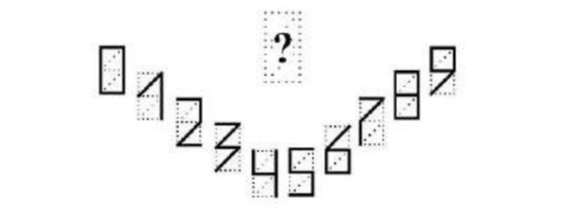
\includegraphics[width=0.8\columnwidth]{pic2.png}
\label{Fig2}
\begin{center}
\caption{ Figure 2. Enumeration of Class Members.}
\end{center}

If all objects of one class have a number of common
properties or features that are absent or have other values
in all representatives of other classes, then the construction of the recognition system can be implemented on the
basis of the principle of generality of properties (\ref{Fig3} Fig. 3).

\includegraphics[width=0.8\columnwidth]{pic03.png}
\begin{center}
\caption{Figure 3. Generality of Properties. }
\label{Fig3}
\end{center}

When the objects of a class are vectors in the feature
space, the class can be considered as a cluster. If clusters
of different classes are separated far enough from each
other, then the construction of the recognition system can
be carried out using the clustering principle \ref{Fic4}(Fig. 4).

\includegraphics[width=0.8\columnwidth]{pic04.png}
\begin{center}
\caption{Figure 4. Clustering}
\label{Fig4}
\end{center}


Traditionally, when building automatic pattern recognition systems, three main problems are solved. The
first one is devoted to the issues of representation of
the initial data obtained as a result of measurements of
the recognized object. The second task is related to the
extraction of essential features and properties from the
initial data. The third one consists in finding optimal
decision rules for classification [18], [19].
\par
In [19], the author, discussing the problem of the
simplicity of the learning process in pattern recognition,
notes the existence of two different approaches to its
implementation. In author’s opinion, in the vast majority
of studies (the first group), the learning process is aimed
at constructing solving rules that ensure the extremum
of a pre-selected criterion. In the second group, the
focus is on understanding the principles of forming
the description of recognition objects, within which the
recognition process becomes extremely simple. Learning
in this case is seen as a process of constructing a space
that is universal, if not for all, then for a wide class of
tasks. Unfortunately, in the author’s opinion, this group
of studies is very few and such an approach to solving
the recognition problem is still poorly studied.
\par
Today, pattern recognition is dominated by an approach in which training is reduced to solving an optimization problem. The training process begins with
the selection of an initial model (a parametric family of
algorithms), and then it is assumed that the "training +
testing” scenario is repeatedly executed. In fact, training
is an iterative process in which positive and negative
reinforcements are used to form the desired patterns of
classifier behavior.
\par
In this case, it should be pointed out that there are
at least two serious problems. First, model selection is a
non-trivial task performed by a data science specialist,
and therefore the training process can be implemented
only in an automated mode. Second, the only result
of training is a classification algorithm, which is an
uninterpretable "black box”.
\par
It is proposed to consider an alternative approach,
when the construction of the classification algorithm is
performed not within the framework of the optimization
problem, but on the basis of the analysis of the properties
of the considered classes. As a result of such analysis, the
distinguishing properties are determined by the mutual
placement of the areas of class definition — patterns.
\par
Before proceeding to the presentation of the alternative
approach, let us consider the classical version of the
mathematical formulation of the recognition problem.
\par
In the paper by Y. I. Zhuravlev [20], the following
formulation of the recognition problem (classification or
Z problem) is given:
\par
 \textit{Let there be a set of admissible objects M. The set is
covered by a finite number of subsets K_{1}, . . . , K_{l}
:  M= \cup^l_{i=1}}
\par
\textit{The main problem (problem Z) is to compute the values
of predicates P_{j} (S) − S ∈ K_{j} , j = 1, 2, . . . , l, from the
information I_{o}(K_{1}, . . . , K_{l})] 
\par and the description of the
admissible object I(S).}

\end{multicols}
\end{document}



